\documentclass{beamer}
\usetheme{Antibes}
\usecolortheme{whale}
\usepackage{latexsym,fancyhdr,amsmath,amsfonts,amsthm,dsfont}
\usepackage{tabularx}
\usepackage{amssymb}
\usepackage{graphicx}
\graphicspath{ {./res/} }
\usepackage{color,latexsym,fancyhdr,amsmath,amsfonts,dsfont,amssymb, amsthm}
%Information to be included in the title page:
\title{NeuraViz: A Web Application For Visualizing Artificial Neural Network Structures}
\author{Bennett Wendorf}
\institute{University of Wisconsin - La Crosse}
\date{April 30, 2024}
 
\begin{document}
 
\frame{\titlepage}

% TODO: Write out presentation notes for each slide (bullet points)

\begin{frame}
    \frametitle{NeuraViz}
    \begin{columns}
        \begin{column}{0.5\textwidth}
            \begin{block}{What is NeuraViz?}
                \begin{itemize}
                    \item What is NeuraViz? \pause
                    \item Why NeuraViz?
                \end{itemize}
            \end{block}
        \end{column}
        \pause
        \begin{column}{0.5\textwidth}
            \begin{itemize}
                \item Breadth of supported models \pause
                \item Ease of use \pause
                \item Portability
            \end{itemize}
        \end{column}
    \end{columns}
\end{frame}

\begin{frame}
    \frametitle{Artificial Neural Networks}
    \begin{block}{}
        What is an artificial neural network?
    \end{block}
    \pause
    \centering
    \includegraphics[scale=0.18]{../01_introduction/res/neural_network.png}
\end{frame}
    
\begin{frame}
    \frametitle{Life Cycle Model}
    \begin{columns}
        \begin{column}{0.5\textwidth}
            \begin{block}{Models}
                \begin{itemize}
                    \item Waterfall
                    \item Iterative
                    \item Agile (Scrum)
                \end{itemize}
            \end{block}
        \end{column}
        \pause
        \begin{column}{0.5\textwidth}
            \includegraphics[scale=0.34]{../02_dev_process/res/sdlc_agile_model.jpg}
            % TODO: Add citation for this
        \end{column}
    \end{columns}
\end{frame}
 
\begin{frame}
    \frametitle{Scrum Tweaks} 
    \begin{itemize}
        \item \textbf{Sprint Length:} \pause 1 week \pause
        \item \textbf{Standups:} \pause weekly \pause
        \item \textbf{Retrospectives:} \pause integrated into standups \pause
        % TODO: Add note to mention that it's still a useful setup despite these changes
    \end{itemize}
\end{frame}

\begin{frame}
    \frametitle{Process Technologies} 
    \centering
    \includegraphics[scale=0.22]{../02_dev_process/res/jira_board_sprint_25.png}
    % TODO: Add notes about what to actually talk about here
    % Point out time tracking
    % Point out item tagging and how it ties into pull requests and other Github features
\end{frame}

\begin{frame}
    \frametitle{Requirements} 
    \begin{columns}
        \begin{column}{0.5\textwidth}
            \begin{block}{Functional Requirements}
                \begin{itemize}
                    \item As a user, I can see the full graph of a valid uploaded model once it finishes processing.
                    \item As a user, I can pan and zoom the model visualization.
                    \item As a user, I can export the graph to \LaTeX{} TikZ syntax.
                    \item Etc.
                \end{itemize}
            \end{block}
        \end{column}
        \pause
        \begin{column}{0.5\textwidth}
            \begin{block}{Non-Functional Requirements}
                \begin{itemize}
                    \item Large network layers are collapsed if they are too big to reasonably render.
                    \item Invalid models are rejected and not stored on the server unnecessarily.
                    \item Etc.
                \end{itemize}
            \end{block}
        \end{column}
    \end{columns}
\end{frame}

\begin{frame}
    \frametitle{Web Application} 
    \centering
    \includegraphics[scale=0.5]{res/client_server.png}
    % TODO: Talk about what each part does at a high level
\end{frame}

\begin{frame}
    \frametitle{Frontend Design} 
    \centering
    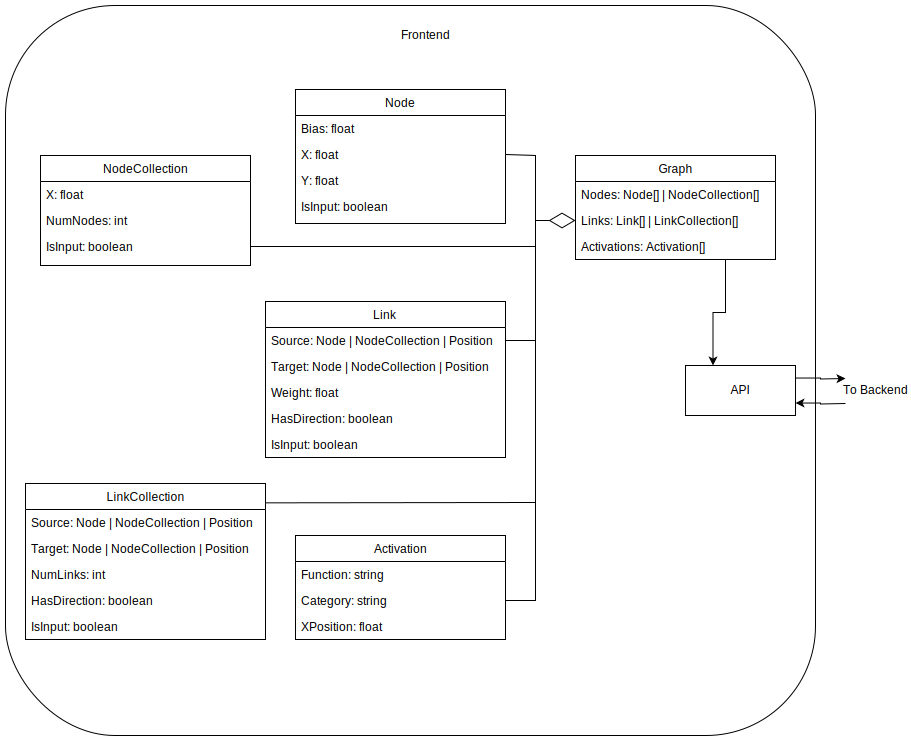
\includegraphics[scale=0.25]{../../docs/diagrams/class_diagram_frontend.png}
    % TODO: What parts of this to touch on?
\end{frame}

\begin{frame}
    \frametitle{Backend Design} 
    \centering
    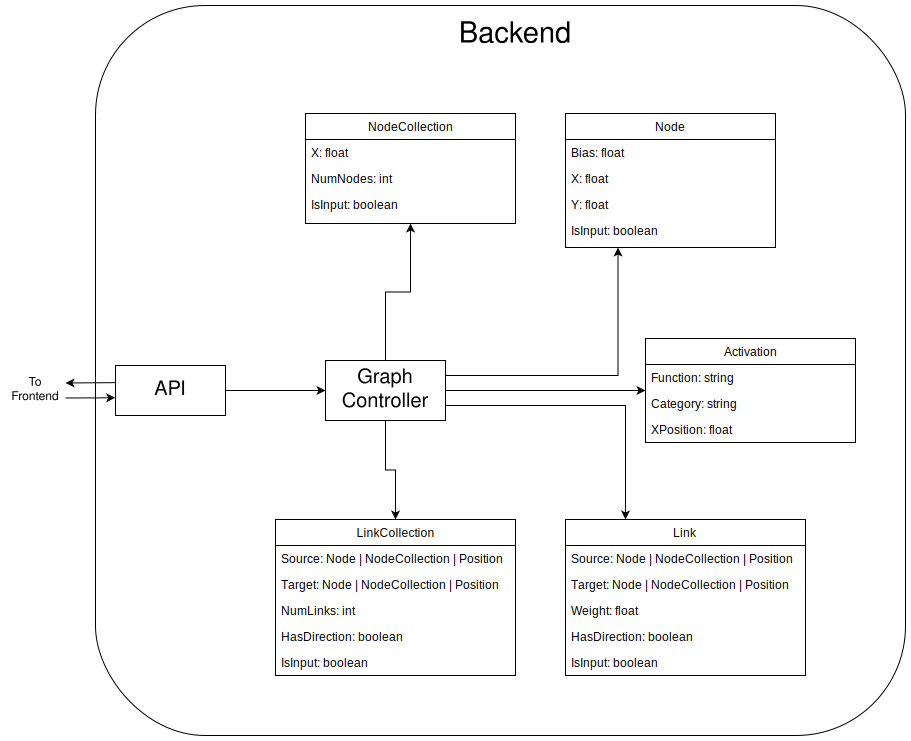
\includegraphics[scale=0.25]{../../docs/diagrams/class_diagram_backend.png}
    % TODO: What parts of this to touch on?
\end{frame}

\begin{frame}
    \frametitle{Database \& Sessions}
    \begin{columns}
        \begin{column}{0.5\textwidth}
            \begin{itemize}
                \item \_id
                \item graphs
                \begin{itemize}
                    \item nodes
                    \item edges
                    \item activations
                \end{itemize}
                \item last\_used
            \end{itemize}
        \end{column}
        \begin{column}{0.5\textwidth}
            \includegraphics[scale=0.125]{res/MongoDB_ForestGreen.png}
            % TODO: Cite from Mongo's website
        \end{column}
    \end{columns}
\end{frame}

\begin{frame}
    \frametitle{User Interface}
    \centering
    \includegraphics[scale=0.15]{../../docs/mockups/Main.png}
\end{frame}

\begin{frame}
    \frametitle{User Interface}
    \centering
    \includegraphics[scale=0.15]{../03_design/res/final_interface.png}
\end{frame}

\begin{frame}
    \frametitle{Frontend Technologies \& Graph Generation}
    \begin{block}{}
        \begin{itemize}
            \item Svelte
            \item Flowbite
            \item D3.js
        \end{itemize}
    \end{block}
    \vspace{0.75cm}
    \centering
    \includegraphics[scale=.25, width=.2\textwidth]{res/svelte_logo.png}\hfill % TODO: Cite https://en.wikipedia.org/wiki/File:Svelte_Logo.svg
    \includegraphics[scale=.05, width=.2\textwidth]{res/flowbite_logo.png}\hfill % TODO: Cite flowbite.com
    \includegraphics[scale=.25, width=.2\textwidth]{res/d3_logo.png} % TODO: Cite https://github.com/d3/d3-logo/blob/master/d3.png
    % TODO: Add notes about graph generation
\end{frame}

\begin{frame}
    \frametitle{Backend Technologies \& Model Parsing}
    % TODO: Add backend tech and model parsing
    \begin{block}{}
        \begin{itemize}
            \item Quart
            \item Keras
            \item PyTorch
        \end{itemize}
    \end{block}
    \vspace{0.75cm}
    \centering
    \includegraphics[scale=.3, width=.2\textwidth]{res/quart_logo.png}\hfill % TODO: Cite https://github.com/koddr/quart-logo/blob/master/src/png/quart_short_logo_color.png
    \includegraphics[scale=.05, width=.2\textwidth]{res/keras_logo.png}\hfill % TODO: Cite https://en.wikipedia.org/wiki/File:Keras_logo.svg
    \includegraphics[scale=.25, width=.2\textwidth]{res/pytorch_logo.png} % TODO: Cite pytorch.com
    % TODO: Add notes about model parsing
\end{frame}

\begin{frame}
    \frametitle{Development}
    % TODO: Should I talk about dev order?
\end{frame}

\begin{frame}
    \frametitle{Deployment}
    % TODO: Talk about deployment
\end{frame}

\begin{frame}
    \frametitle{Testing}
    % TODO: Talk about testing (All 3 types)
\end{frame}

\begin{frame}
    \frametitle{Security}
    % TODO: Talk about security
\end{frame}

\begin{frame}
    \frametitle{Challenges}
    % TODO: Talk about challenges
\end{frame}

\begin{frame}
    \frametitle{Future Work}
    % TODO: Talk about future work
\end{frame}

\begin{frame}
    \frametitle{Thank you}
    Questions
    \centering
\end{frame}

\end{document}
